
\begin{frame}[fragile]{MiniBrass}

\begin{center}


\includegraphics[width=.5\textwidth]{img/minibrass.png}

\vspace*{2ex}

\url{http://isse-augsburg.github.io/minibrass/}

\end{center}

\end{frame}

\begin{frame}[fragile]{MiniBrass: HelloWorld}
\begin{columns}[onlytextwidth,T]
    
    \begin{column}{.40\textwidth}
          
    \hSecond{Basismodell (MiniZinc)}
    \begin{lstlisting}
include "hello_o.mzn"; 
include "soft_constraints/
   pvs_gen_search.mzn"; 
% the basic, "classic" CSP 
set of int: DOM = 1..3;

var DOM: x; var DOM: y; 
var DOM: z;
% add. *hard* constraints
% e.g. constraint x < y;

solve search pvs_BAB();
\end{lstlisting}
    \end{column}
    
    \begin{column}{.55\textwidth}
  	\hFirst{Präferenzmodell (MiniBrass)} 
  	\begin{lstlisting}
PVS: cr1 = 
  new ConstraintRelationships("cr1") {
   soft-constraint c1: 'x + 1 = y';
   soft-constraint c2: 'z = y + 2';
   soft-constraint c3: 'x + y <= 3';
   
   crEdges : '[| mbr.c2, mbr.c1 | 
                  mbr.c3, mbr.c1 |]';
   useSPD: 'true' ;
}; 

solve cr1;
\end{lstlisting}

    \end{column}
  \end{columns}
  \pause
  \begin{verbatim}
Solution:  x = 1; y = 2; z = 1
Valuations:  mbr_overall_cr1 = {c2}
----------
==========
  \end{verbatim}
  \begin{textblock*}{3cm}[1,1](\textwidth+0.5cm,\textheight-0.3cm)
%\textblockcolour{issegrey!20}
\begin{center}
\begin{tikzpicture}[auto,
                    ->,>=stealth',shorten >=1pt,thick,
                    node distance=.7cm,inner sep=2pt,
                    constraint/.style={circle,fill=black!15,draw,font=\sffamily\small}]
\node[constraint node] (1) at (0, 0)                   {$\mathrm{c}_1$};
\node[constraint node] (2) at ($ (1) + (-0.8, -0.8) $) {$\mathrm{c}_2$};  
\node[constraint node] (3) at ($ (1) + ( 0.8, -0.8) $) {$\mathrm{c}_3$};  
%  
\path[every node/.style={font=\sffamily\tiny}]
  (2) edge (1)
  (3) edge (1)
  ;
  

\end{tikzpicture}
\end{center}
\end{textblock*}
\end{frame}


\begin{frame} \small
\frametitle{Single-Predecessor-Dominance (SPD) Lifting}

\cemph{isWorseThan}-Relation für Mengen verletzter Constraints~\cite{Schiendorfer13}
%
\bgroup\abovedisplayskip=4pt\belowdisplayskip=12pt
\begin{gather*}
  V \uplus \{ c \}  \supset_{\mathsf{SPD}}  V 
\\
  V \uplus \{ c_{\mathrm{gold}} \}  \supset_{\mathsf{SPD}}  V \uplus \{ c_{\mathrm{silber}} \}
\quad\text{wenn $c_{\mathrm{silber}}$ weniger wichtig als $c_{\mathrm{gold}}$}
\end{gather*}
\egroup

\begin{center}
\begin{tikzpicture}[auto,
                    ->,>=stealth',shorten >=1pt,thick,
                    node distance=1cm,inner sep=2pt,
                    constraint/.style={circle,fill=black!15,draw,font=\sffamily\small}]
\begin{scope}
\node[constraint,fill=green] (1) at (0, 0)                   {$\mathrm{c}_7$};
\node[constraint,fill=red] (2) at ($ (1) + (-1.2, -0.8) $) {$\mathrm{c}_4$};  
\node[constraint,fill=green]   (3) at ($ (2) + (0.0, -0.9) $) {$\mathrm{c}_5$};  
\node[constraint,fill=green] (4) at ($ (3) + ( 0.0, -1.0) $) {$\mathrm{c}_6$};
\node[constraint,fill=green] (7) at ($ (1) + ( 1.2, -0.8) $) {$\mathrm{c}_1$};  
\node[constraint,fill=red]   (8) at ($ (7) + (-0.6, -0.9) $) {$\mathrm{c}_2$};  
\node[constraint,fill=red]   (9) at ($ (7) + ( 0.6, -0.9) $) {$\mathrm{c}_3$};  
%  
\path[every node/.style={font=\sffamily\tiny}]
  (2) edge (1)
  (7) edge (1)
  (3) edge (2)
  (4) edge (3)
  (8) edge (7)
  (9) edge (7)
  ;
\end{scope}
%
\begin{scope}[xshift=6cm]
\node[constraint,fill=green] (1) at (0, 0)                   {$\mathrm{c}_7$};
\node[constraint,fill=green]   (2) at ($ (1) + (-1.2, -0.8) $) {$\mathrm{c}_4$};  
\node[constraint,fill=red] (3) at ($ (2) + (0.0, -0.9) $) {$\mathrm{c}_5$};  
\node[constraint,fill=green] (4) at ($ (3) + ( 0.0, -1.0) $) {$\mathrm{c}_6$};  
\node[constraint,fill=green] (7) at ($ (1) + ( 1.2, -0.8) $) {$\mathrm{c}_1$};  
\node[constraint,fill=red]   (8) at ($ (7) + (-0.6, -0.9) $) {$\mathrm{c}_2$};  
\node[constraint,fill=red]   (9) at ($ (7) + ( 0.6, -0.9) $) {$\mathrm{c}_3$};  
%  
\path[every node/.style={font=\sffamily\tiny}]
  (2) edge (1)
  (7) edge (1)
  (3) edge (2)
  (4) edge (3)
  (8) edge (7)
  (9) edge (7)
  ;
\end{scope}
%
\node (R) at (3.05, -1.4) {$ \supset_{\mathsf{SPD}}$};
\end{tikzpicture}
\end{center}

\begin{itemize}
\item Bekannt als \emph{Smyth-Ordnung} (Powerdomains) \hfill \cite[Ch.~9]{amadio-curien:1998}
\item Entsteht aus \emph{freier Konstruktion} über Constraint-Relationship.\hfill \cite{knapp-schiendorfer2014ictai}
\end{itemize}

%
%\cemph{Ordnungs}relation über Zuweisungen 
%\bgroup\abovedisplayskip4pt
%\begin{equation*}
%  w \SPDord{R} v \iff \{ c \in C \mid v \not\models c \} \mathrel{({\SPDrel{R}})^{+}} \{ c \in C \mid w \not\models c \}
%\end{equation*}
%\egroup

\end{frame}

\tikzset{onslide/.code args={<#1>#2}{%
  \only<#1>{\pgfkeysalso{#2}}
}}
\tikzstyle{highlight}=[isseorange,ultra thick]
\tikzstyle{highlight2}=[CornflowerBlue,ultra thick]
\begin{frame}[fragile]{Constraint-Optimierung mit PVS}
Der partiell geordnete Bewertungsraum



\begin{figure}[!t]
\begin{center}
\begin{tikzpicture}[scale=0.77,auto]

% single PVS
\node (bot) at (0,0) {\alert{$\bot = \{c_1, c_2, c_3 \}$}};
\node (c1c2) at (-2,1) {\alert<2->{$\{c_1, c_2\}$}};
\node (c2c3) at (0,2) {$\{c_2, c_3\}$};
\node (c1c3) at (2,1) {$\{c_1, c_3\}$};

\node (c1) at (0,3) {\alert<3->{$\{c_1\}$}};
\node (c2) at (-2,4) {\alert<4->{$\{c_2\}$}};
\node (c3) at (2,4) {$\{c_3\}$};
%\node (a) at (-1,0.5) {$a$};
%\node (b) at (-1,1.5) {$b$};
%\node (c) at (1,1) {$c$};
\node (top) at (0,5) {$\top = \emptyset$};

\node[text width=2cm] (verb) at (4,0) {     };
\path[-]
(bot) edge[onslide={<2->{highlight}}] (c1c2)
      edge (c2c3)
      edge (c1c3)
(c1c2) edge (c2c3)
(c1c3) edge (c2c3)
(c1c3) edge (c1)
(c1c3) edge (c3)
(c2c3) edge (c2)
(c2c3) edge (c3)
(c1c2) edge[onslide={<3->{highlight}}] (c1)
(c1c2) edge (c2)
(c1) edge[onslide={<4->{highlight}}] (c2)
(c1) edge (c3)
(c2) edge (top)
(c1) edge (top)
(c3) edge (top)
      ;
%(a) edge (b)
%(b) edge (top)
%(bot) edge (c)
%(c) edge (top)
;

\end{tikzpicture}
\end{center}
\label{fig:nosuprema}
\end{figure}
\begin{lstlisting}
function ann: pvs_BAB() =
       repeat(
           if next() then 
                 print("Intermediate solution:") /\ print() /\
                 commit() /\ postGetBetter()
           else break endif       );
\end{lstlisting}
\begin{textblock*}{2.5cm}[1,1](\textwidth-8.8cm,\textheight-4.03cm)
\begin{tikzpicture}[auto,
                    ->,>=stealth',shorten >=1pt,thick,
                    node distance=.7cm,inner sep=2pt,
                    constraint/.style={circle,fill=black!15,draw,font=\sffamily\small}]
\node[constraint node] (1) at (0, 0)                   {$\mathrm{c}_1$};
\node[constraint node] (2) at ($ (1) + (-0.8, -0.8) $) {$\mathrm{c}_2$};  
\node[constraint node] (3) at ($ (1) + ( 0.8, -0.8) $) {$\mathrm{c}_3$};  
%  
\path[every node/.style={font=\sffamily\tiny}]
  (2) edge (1)
  (3) edge (1)
  ;
  

\end{tikzpicture}
\begin{Verbatim}[fontsize=\small]
c1: 'x + 1 = y';
c2: 'z = y + 2';
c3: 'x + y <= 3';   
\end{Verbatim}
\end{textblock*}

\begin{textblock*}{4cm}[1,1](\textwidth+0.5cm,\textheight-3.03cm)

\onslide<2->{

{ \tt  \small
x = 1; y = 1; z = 1 \newline
Valuation = \{c1,c2\}
}
}

\onslide<3->{
{ \tt  \small
----------

x = 1; y = 1; z = 3 \newline
Valuation = \{c1\}
}
}


\onslide<4->{
{ \tt  \small
----------

x = 1; y = 2; z = 1 \newline
Valuations = \{c2\}

----------

==========

}
}
\end{textblock*}
\end{frame}

\tikzset{
    process/.style={rectangle,rounded corners,draw=black, top color=isseorange!5, bottom color=isseorange!30},
    file/.style={rectangle,draw=black}
}
\begin{frame}{MiniBrass: Workflow} \small

\vspace*{-2ex}
\alert{Architektur}

\begin{center}
\vspace*{-10ex}
\begin{tikzpicture}[>=stealth,auto,every node/.style={
anchor=base,
text depth=.5ex,
text height=2ex,
minimum height=2ex,
align=center,
circle,
minimum width=1em}]
\matrix (magic) [nodes in empty cells, ampersand replacement=\&,row sep=0.5cm,column sep=0.5cm]
{
\node{}; \&\node[draw, file,isseorange,thick](mbrlibs){\texttt{mbrlibs.mzn}}; \& \& \node[draw, file,isseorange,thick](types){\texttt{types.mbr}}; \\
\node {};\& \node[draw, file,CornflowerBlue,thick](mbr){\texttt{prefs.mbr}};   \& \& \node[draw, isseorange,thick,process](mbr2mzn){\texttt{mbr2mzn}}; \\
\node {};\& \& \& \node[draw, file,isseorange,thick](compiledMzn){\emph{prefs\_o.mzn}}; \\
%    \&  \&  \node(inv){}; \&  \\
\node {};\& \node[draw, file,CornflowerBlue!80](f1){\texttt{model.mzn}}; \& \& \node[draw, process](mzn2fzn){\texttt{mzn2fzn}}; \& \& \node[draw, file](output){\emph{output}};  \\
%    \&  \&  \node(inv){}; \&  \\
\node {};\& \node[draw, file,CornflowerBlue!80](mod){\texttt{data.dzn}}; \& \&  \\
\node {};\& \node[draw, file](mznlibs){\texttt{mznlibs.mzn}};\& \& \node[draw, file](fzn){\texttt{compiled.fzn}}; \& \& \node[draw, process](solve){\texttt{solve}};  \\
\node {};\& \& \\
};

\draw[dashed,->] (f1) -- (mzn2fzn);
\draw[dashed,->] (mbr) -- (mbr2mzn);
\draw[dashed,->] (mod) -- (mzn2fzn);
\draw[dashed,-] (types) -- (mbrlibs);
\draw[dashed,-] (types) -- (mbr);
%\draw[dashed,->] (mbrlibs) -- (mzn2fzn);
%\draw[dashed] (mbrlibs) -- (mbr);
\draw[dashed,->] (compiledMzn) -- (mzn2fzn);
\draw[dashed,->] (mznlibs) -- (mzn2fzn);
\draw[dashed,->] (fzn) -- (solve);
\draw[->] (mbr2mzn) -- (compiledMzn);

\draw[->] (mzn2fzn) -- (fzn);
\draw[->] (solve) -- (output);
%\draw[dashed] (globals) -- (inv);

%\onslide<4->{  
%\node[overlay,align=left,rectangle callout,%
%      callout absolute pointer=(mbrlibs.west),fill=CornflowerBlue!50] at (-4.5,5) {PVS-Prädikate};}

\onslide<4->{  
\node[overlay,align=left,rectangle callout,%
      callout absolute pointer=(mbrlibs.north),fill=isseorange!50] at (-3,7.5) {Implementierte Funktionen und Prädikate};}
            
\onslide<3->{  
\node[overlay,align=left,rectangle callout,%
      callout absolute pointer=(types.north),fill=isseorange!50] at (2,7.5) {PVS-Typdefinitionen};} 
     
\onslide<3->{  
\node[overlay,align=left,rectangle callout,%
      callout absolute pointer=(mbr.west),fill=CornflowerBlue!50] at (-3.7,4.5) {PVS-Instanzen, Kombinationen};} 
     
\end{tikzpicture}
\end{center}
\vspace*{-25ex}

\end{frame}


\begin{frame}[fragile]{PVS-Typdefinitionen}
\begin{lstlisting}
type ConstraintRelationships = PVSType<bool, set of 1..nScs> = 
  params { 
    array[int, 1..2] of 1..nScs: crEdges; % adjacency matrix
    bool: useSPD;
  } in 
  instantiates with "../mbr_types/cr_type.mzn" {
    times -> link_invert_booleans;
    is_worse -> is_worse_cr;
    top -> {};
  };
\end{lstlisting}
\begin{itemize}
\item \texttt{PVSType<S,E>} Unterscheidet zur einfacheren Verwendung zwischen 
\begin{itemize}
\item[] Spezifikationstyp $S$ 
\item[] Elementtyp $E$
\end{itemize} 
\item Kombinationsoperation: $\mathtt{times} : S^n \to E$
\item Ordnungsrelation: $\mathtt{isWorse} \subseteq E \times E$
\end{itemize}
\end{frame}

%\begin{frame}[fragile]{PVS-Definitionen}
%Innerhalb von \texttt{../mbr\_types/cr\_type.mzn}:
%\begin{lstlisting}
%function var set of int: 
%  link_invert_booleans(array[int] of var bool: b...
%
%% gives us access to constraint relationship predicates 
%include "soft_constraints/spd_worse.mzn";
%include "soft_constraints/tpd_worse.mzn";
%
%predicate is_worse_cr(var set of int: violated1, 
%                      var set of int: violated2,
%                      par int: nScs, array[int, 1..2] of par int: crEdges, 
%                      par bool: useSPD) =
%let {  par set of int: softConstraints = 1..nScs; } in (                    
%    if useSPD then
%      spd_worse(violated1, violated2, softConstraints, crEdges)
%    else
%      tpd_worse(violated1, violated2, softConstraints, crEdges)
%    endif);
%
%\end{lstlisting}
%\end{frame}

\begin{frame}[fragile]{PVS-Instanziierung (Revisited)}
\begin{lstlisting}
PVS: cr1 = new ConstraintRelationships("cr1") {
   soft-constraint c1: 'x + 1 = y';
   soft-constraint c2: 'z = y + 2';
   soft-constraint c3: 'x + y <= 3';
   
   crEdges : '[| mbr.c2, mbr.c1 | mbr.c3, mbr.c1 |]';
   useSPD: 'false' ;
}; 
\end{lstlisting}
\begin{itemize}
\item Jeder Soft-Constraint ein $S$-Ausdruck (hier z.B. $\mathtt{bool}$)
\item Mittels der Funktion $\mathtt{times}$ auf einen $E$-Wert abgebildet
\item Ausdrücke in einfachen Anführungszeichen: \alert{MiniZinc}-Code (nicht geparst, bis auf \texttt{mbr.}-Präfixe)
\item Parameter aus \texttt{PVSType} müssen Wert erhalten
\end{itemize}
\end{frame}

\begin{frame}[fragile]{Weitere PVS-Typen}
\begin{lstlisting}
type WeightedCsp = PVSType<bool, int> = 
  params {
    int: k; 
    array[1..nScs] of 1..k: weights :: default('1');
  } in  
  instantiates with "../mbr_types/weighted_type.mzn" {
    times -> weighted_sum;
    is_worse -> is_worse_weighted;
    top -> 0;
  };
  
type CostFunctionNetwork = PVSType<0..k> = 
  params {
    int: k :: default('1000'); 
  } in  instantiates with "../mbr_types/cfn_type.mzn" {
    times -> sum;
    is_worse -> is_worse_weighted; 
    top -> 0;
 };
\end{lstlisting}
\end{frame}

\begin{frame}[fragile]{PVS-Instanziierung Weighted}
\begin{lstlisting}
PVS: cr1 = new WeightedCsp("cr1") {
   soft-constraint c1: 'x + 1 = y' :: weights('2');
   soft-constraint c2: 'z = y + 2' :: weights('1');
   soft-constraint c3: 'x + y <= 3' :: weights('1');
   
   k : '20';
}; 
\end{lstlisting}
\begin{itemize}
\item Gewichte können direkt an Soft Constraints annotiert werden
\item Oder direkt als Feld übergeben werden (\texttt{[2,1,1]}) %\item Aber können wir sie nicht auch berechnen? Aus Constraint Relationships? \pause 
\end{itemize}
\end{frame}

\begin{frame}{Übergang zwischen PVS-Typen}\small

\begin{itemize}
\item Unter Umständen wollen wir zwischen PVS-Typen \emph{übersetzen} können 
%
\begin{itemize}
\item[-] Ordnung soll bewusst totalisiert werden (z.B. sonst unübersichtlich)
\item[-] Datentyp $xy$ (z.B. Mengen) wird von Solver/Algorithmus nicht unterstützt (häufig in math. Prog.)
\item[-] $\rightarrow$ Benutzer interessiert \alert{nicht} konkrete Datenstruktur sondern nur die Erhaltung der gewünschten Ordnung
\item[-] Beispiel: Gewichte aus Constraint Relationships für CPLEX
\end{itemize}
%
\vspace*{2ex}
\item Daher suchen wir nach \emph{strukturerhaltenden} Abbildungen \pause
\item PVS-Homomorphismus $\varphi : \mathsf{PVS}_{\mathrm{cr}} \to  \mathsf{PVS}_{\mathrm{weighted}}$ \pause 
\item $\mathsf{PVS}_{\mathrm{cr}} = \mathit{PVS}\langle P \rangle = \langle \mathcal{M}^{\mathrm{fin}} (P), \mcup, \supseteq_{\mathsf{SPD}}, \lbag \rbag \rangle$
\begin{itemize}
\item[-] $\varphi(\top_{\mathrm{cr}}) = \top_{\mathrm{weighted}}$ \pause 
\item[-] $\varphi(m \cdot_{\mathrm{cr}} n) = \varphi(m) \cdot_{\mathrm{weighted}} \varphi(n)$ \pause 
\item[-] $m \leq_{\mathrm{cr}} n \rightarrow \varphi(m) \leq_{\mathrm{weighted}} \varphi(n)$ \pause 
\end{itemize}

\end{itemize}
%\begin{center}
%\begin{tikzpicture}
%  \matrix (m) [matrix of math nodes,row sep=3em,column sep=4em,minimum width=2em,ampersand replacement=\&]
%  {
%     \mathit{PVS}\langle P \rangle  \&  \mathit{Weighted}(P) \&  \\
%  };
%      
%  \path[-stealth]
%    (m-1-1) edge node [above] {$\SPDw{}$} (m-1-2)
%;
%
%\end{tikzpicture}
%\end{center}
\begin{textblock*}{3cm}[1,1](\textwidth+.5cm,\textheight-1.3cm)
%\textblockcolour{issegrey!20}
\begin{center}
\begin{tikzpicture}[auto,
                    ->,>=stealth',shorten >=1pt,thick,
                    node distance=.7cm,inner sep=2pt,
                    constraint/.style={circle,fill=black!15,draw,font=\sffamily\small}]
\node[overlay,rectangle callout,callout absolute pointer = {(-3,0.8)},
     draw=isseorange!50,fill=white] at (0,.5) {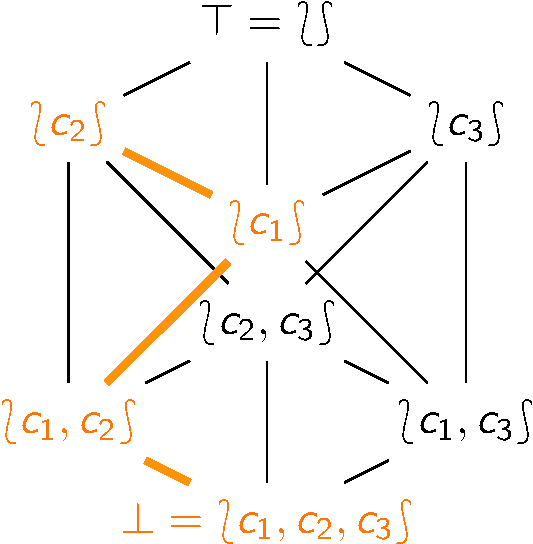
\includegraphics[width=2cm]{img/search-space.pdf}};  
\end{tikzpicture}

\end{center}
\end{textblock*}
\end{frame}

\begin{frame}{Bsp.: Gewichte für Constraint Relationships}
\begin{figure}
\centering
\begin{tikzpicture}[->,>=stealth',shorten >=1pt,auto,node distance=1.45cm,inner sep=1.5pt,outer sep = 0.0pt, thick] 

\tikzstyle{every node}=[font=\small]

\begin{scope}[xshift=-12cm,yshift=0.0cm]
\node[constraint node, xshift=0.6cm, label=west:{\small 4/13}] (1) {$\mathrm{c_7}$};
\node[constraint node, xshift=1cm, label=east:{\small 2/3}] (3)  [below right of=1] {$\mathrm{c_1}$};
\node[constraint node, label=0:{\small 1/1}] (4) [below left of=3] {$\mathrm{c_2}$};
\node[constraint node, label=0:{\small 1/1}] (8) [below right of=3] {$\mathrm{c_3}$};
\node[constraint node, label=0:{\small 3/4}] (5) [below left of=1, xshift=-.5cm] {$\mathrm{c_4}$};
\node[constraint node, node distance=0.85cm, label=0:{\small 2/2}] (6) [below of=5] {$\mathrm{c_5}$};  
\node[constraint node, node distance=0.85cm,label=0:{\small 1/1}] (7) [below of=6] {$\mathrm{c_6}$};  

\path[every node/.style={font=\sffamily\tiny}]
  (3) edge node [right] {} (1)
  (5) edge node [right] {} (1)
  (4) edge node [right] {} (3)
  (8) edge node [right] {} (3) 	
  (6) edge node [right] {} (5)
  (7) edge node [right] {} (6)    
  ;
        
%\draw [rounded corners, black!45,dashed] (-2.0,-0.5) rectangle (0.3,-3.8);
%\node[yshift=-.75cm] (ag1) at (7){ Agent 1};
    
%\draw [rounded corners, black!45,dashed] (0.6,-0.5) rectangle (4.5,-3.8);
%\node[yshift=-2.45cm] (ag2) at (3) { Agent 2};
\end{scope}

\end{tikzpicture}
\caption{Beispiel mit errechneten Gewichten (SPD/TPD)}
\label{fig:combRelGraph}
\end{figure}


%%% Local Variables:
%%% mode: LaTeX
%%% mode: TeX-PDF
%%% mode: TeX-source-correlate
%%% TeX-master: "../quality-quantity-soft-constraints.tex"
%%% End:


\bgroup\abovedisplayskip=-16pt\belowdisplayskip=4pt
\begin{align*}
  \SPDw{}(c) &\textstyle= 1 + \max_{c' \rightarrow^+ c} \SPDw{}(c') 
\\
  \TPDw{}(c) &\textstyle= 1 + \sum_{c' \rightarrow^+ c} \TPDw{}(c')  
\end{align*}
\egroup

\vspace*{1ex} \small \pause 
\begin{itemize}
\item Für Ordnung $P$ über Constraints: PVS $\mathrm{Weighted}(P) = \langle \mathbb{N}, +, \geq, 0 \rangle$
\item $\mathsf{PVS}_{\mathrm{cr}} = \mathit{PVS}\langle P \rangle = \langle \mathcal{M}^{\mathrm{fin}} (P), \mcup, \supseteq_{\mathsf{SPD}}, \lbag \rbag \rangle$
\item $\varphi(\lbag \rbag) = 0$, $\varphi(\lbag c\rbag \mcup C) = \SPDw{}(c) + \varphi(C)$
\end{itemize}



\hfill \cite{Schiendorfer13}
\begin{textblock*}{3cm}[1,1](\textwidth+1cm,\textheight-2.7cm)
%\textblockcolour{issegrey!20}
\begin{center}
\begin{tikzpicture}[auto,
                    ->,>=stealth',shorten >=1pt,thick,
                    node distance=.7cm,inner sep=5pt, 
                    constraint/.style={circle,fill=black!15,draw,font=\sffamily\small}]
\node[overlay,rectangle callout,callout absolute pointer = {(-2,-1)},
     draw=isseorange!50,fill=white] at (0,0) {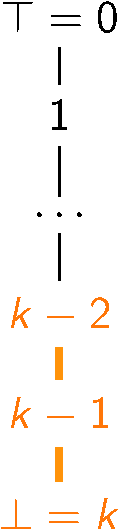
\includegraphics[width=.6cm]{img/search-space-weighted.pdf}};  
\end{tikzpicture}
\end{center}
\end{textblock*}
\end{frame}
%
%\begin{frame}{PVS und Morphismen} \small
%Etwas systematischer \ldots 
%\begin{itemize}
%\item $\mathsf{PVS}_{\mathrm{cr}} = \mathit{PVS}\langle P \rangle = \langle \mathcal{M}^{\mathrm{fin}} (P), \mcup, \supseteq_{\mathsf{SPD}}, \lbag \rbag \rangle$
%\item PVS-Homomorphismus $\varphi : \mathsf{PVS}_{\mathrm{cr}} \to  \mathsf{PVS}_{\mathrm{weighted}}$ \pause 
%\begin{itemize}
%\item[-] $\varphi(\top_{\mathrm{cr}}) = \top_{\mathrm{weighted}}$ \pause 
%\item[-] $\varphi(m \cdot_{\mathrm{cr}} n) = \varphi(m) \cdot_{\mathrm{weighted}} \varphi(n)$ \pause 
%\item[-] $m \leq_{\mathrm{cr}} n \rightarrow \varphi(m) \leq_{\mathrm{weighted}} \varphi(n)$ \pause 
%\end{itemize}
%
%\vspace*{2ex}
%
%\item Beispiel: $\varphi(\lbag \rbag) = 0$, $\varphi(\lbag c\rbag \mcup C) = \SPDw{}(c) + \varphi(C)$
%
%\vspace*{2ex}
%
%\pause 
%\item Warum überhaupt Morphismen?
%\begin{itemize}
%\item[-] Ordnung soll bewusst totalisiert werden
%\item[-] Datentyp $xy$ (z.B. Mengen) wird von Solver/Algorithmus nicht unterstützt
%\item[-] $\rightarrow$ Benutzer interessiert \alert{nicht} konkrete Datenstruktur sondern nur die Erhaltung der gewünschten Ordnung
%\end{itemize}
%\end{itemize}
%%\begin{center}
%%\begin{tikzpicture}
%%  \matrix (m) [matrix of math nodes,row sep=3em,column sep=4em,minimum width=2em,ampersand replacement=\&]
%%  {
%%     \mathit{PVS}\langle P \rangle  \&  \mathit{Weighted}(P) \&  \\
%%  };
%%      
%%  \path[-stealth]
%%    (m-1-1) edge node [above] {$\SPDw{}$} (m-1-2)
%%;
%%
%%\end{tikzpicture}
%%\end{center}
%\begin{textblock*}{3cm}[1,1](\textwidth+.5cm,\textheight-5.3cm)
%%\textblockcolour{issegrey!20}
%\begin{center}
%\begin{tikzpicture}[auto,
%                    ->,>=stealth',shorten >=1pt,thick,
%                    node distance=.7cm,inner sep=2pt,
%                    constraint/.style={circle,fill=black!15,draw,font=\sffamily\small}]
%\node[overlay,rectangle callout,callout absolute pointer = {(-3,0.8)},
%     draw=isseorange!50,fill=white] at (0,.5) {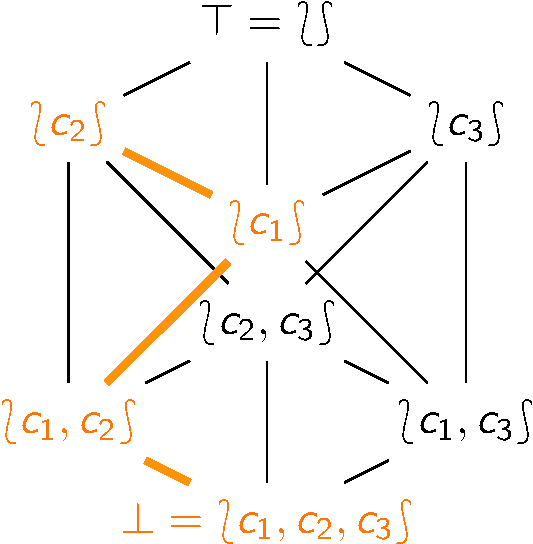
\includegraphics[width=2cm]{img/search-space.pdf}};  
%\end{tikzpicture}
%
%\end{center}
%\end{textblock*}
%\end{frame}


\begin{frame}{Looking for freedom \ldots} \small

\begin{center}
\begin{tikzpicture}[auto,->,
                    >=stealth',shorten >=1pt,thick,
                    node distance=.7cm,inner sep=2pt,
                    constraint/.style={circle,fill=black!15,draw,font=\sffamily\small},
                    bg/.style={shape=rectangle, rounded corners,
    draw, align=center,
    top color=white, bottom color=issegrey!15},
                    pvs/.style={shape=rectangle, rounded corners,
    draw=isseorange!50,fill=white, align=center}]
\node [anchor=west] at (0, .5) {$\mathrm{Cat}: \mathrm{POSet}$};
\node [anchor=west] at (0, -.5) {$\mathrm{Cat}: \mathrm{PVS}$};

\draw [dashed,-] (0,0) -- (11,0);

 \node[bg,text width=2.7cm, text height=1.5cm] at (5,1.6) {};
 \node[anchor=west] at (3.6,2.1) {$P$};
 
\node[constraint node] (1) at (5, 2)                   {$\mathrm{c}_1$};
\node[constraint node] (2) at ($ (1) + (-0.8, -0.8) $) {$\mathrm{c}_2$};  
\node[constraint node] (3) at ($ (1) + ( 0.8, -0.8) $) {$\mathrm{c}_3$};  
%  
\path[every node/.style={font=\sffamily\tiny}]
  (2) edge (1)
  (3) edge (1)
  ;
 
\onslide<2-> { 
\node[pvs,text width=3.5cm,anchor=north west, text height=2.8cm] at (0.5,-1) {};
 \node[anchor=west] at (0.5,-1.3) {$\mathit{Weighted}(P)$};
  \node[anchor=west] at (0.5,-3.6) {$\langle \mathbb{N}, +, \geq, 0 \rangle$};
  
\node[constraint node,label=west:2] (w1) at (2, -2)                   {$\mathrm{c}_1$};
\node[constraint node,label=west:1] (w2) at ($ (w1) + (-0.8, -0.8) $) {$\mathrm{c}_2$};  
\node[constraint node,label=west:1] (w3) at ($ (w1) + ( 0.8, -0.8) $) {$\mathrm{c}_3$};  
\node at (3.5, -2.3) {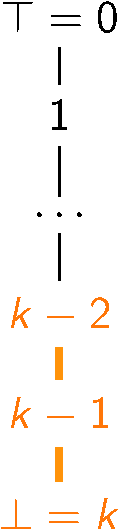
\includegraphics[width=.45cm]{img/search-space-weighted.pdf} }; 

%  
\path[every node/.style={font=\sffamily\tiny}]
  (w2) edge (w1)
  (w3) edge (w1)
  ;
}

\onslide<3->{
\draw [CornflowerBlue] (5,0.7) -- (2,-1);
\node [CornflowerBlue] at (4.2,-0.5) {$\mu(c) = \SPDw{}(c)$};
}  
 
\onslide<4->{
\node[pvs,text width=4.5cm,anchor=north west, text height=2.8cm] at (5.7,-1) {};
\node[anchor=west] at (5.7,-1.3) {$\mathit{PVS}\langle P \rangle $};
\node[anchor=west] at (5.7,-3.6) {$\langle \mathcal{M}^{\mathrm{fin}} (P), \mcup, \smytheq{P}, \lbag \rbag \rangle$};

\node[constraint node,label=west:$\lbag \mathrm{c}_1 \rbag$] (p1) at (7, -2)                   {$\mathrm{c}_1$};
\node[constraint node,label=east:$\lbag \mathrm{c}_2 \rbag$] (p2) at ($ (p1) + (-0.8, -0.8) $) {$\mathrm{c}_2$};  
\node[constraint node,label=north:$\lbag \mathrm{c}_3 \rbag$] (p3) at ($ (p1) + ( 0.8, -0.8) $) {$\mathrm{c}_3$};  
\node at (9.2, -2.3) {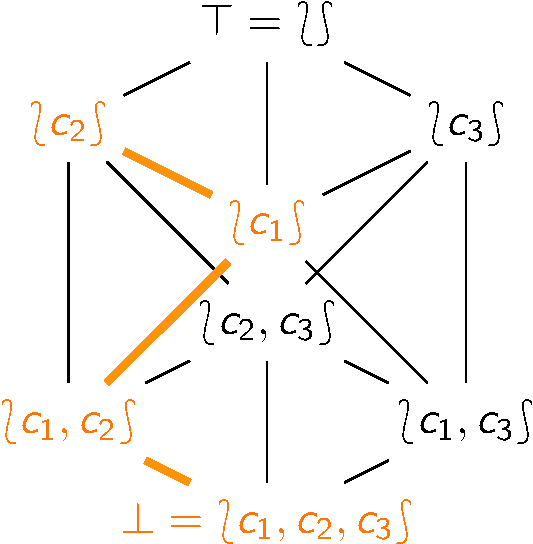
\includegraphics[width=2cm]{img/search-space.pdf} }; 
%  
\path[every node/.style={font=\sffamily\tiny}]
  (p2) edge (p1)
  (p3) edge (p1)
  ;
}
 
\onslide<5->{ 

\draw [isseorange] (5,0.7) -- (8,-1);
\node [isseorange] at (8.7,-0.5) {$\eta(c) = \lbag c \rbag$};
}

\onslide<6->{
\draw [issegrey] (5.7,-2) to [bend right] (4.2,-2);  
\node [issegrey] at (5,-1.5) {$(\SPDw{})^\#$};
}

\onslide<7->{
\draw [issegrey]  (4.2,-2.5) to [bend right] (5.7,-2.5);   
\node [issegrey] at (5,-3) {?};
}
\end{tikzpicture}
\end{center}

\end{frame}

\begin{frame}{Looking for freedom \ldots}
%\begin{itemize}
%\item (Konkrete) Kategorie $\mathsf{POSet}$: 
%\begin{itemize}
%\item[-] Objekte $\rightarrow$ partiell geordnete Mengen
%\item[-] Morphismen $\rightarrow$ monotone Funktionen
%\end{itemize}  
%\end{itemize}
\begin{lemma}[PVS-Freiheit \cite{knapp-schiendorfer2014}]
$\mathit{PVS}\langle P \rangle$ is the free partial valuation structure over the partial order $P$.
\end{lemma}


\begin{center}
\begin{tikzpicture}
  \matrix (m) [matrix of math nodes,row sep=3em,column sep=4em,minimum width=2em,ampersand replacement=\&]
  {
     P \& \mathit{PO}(\mathit{PVS}\langle P \rangle) \& \& \mathit{PVS}\langle P \rangle \\
      \& \mathit{PO}(M) \& \& M \\};
  \path[-stealth]
    (m-1-1) edge node [above] {$\eta_P^{\mathrm{PVS}}$} (m-1-2)
            edge node [below left] {$\varphi$} (m-2-2)
    (m-1-2) edge node [right] {$\mathit{PO}( \varphi^{\# \mathrm{PVS} })$} (m-2-2)
    (m-1-4) edge [dashed] node [right] {$\varphi^{\# \mathrm{PVS} }$} (m-2-4)
;
\end{tikzpicture}
\end{center}

\cemph{Freie Konstruktionen}

\begin{itemize}
\item no junk
\item no confusion
\end{itemize}
\end{frame}

\begin{frame}[fragile]{Morphismen in MiniBrass}
\begin{lstlisting}
% aus Bibliothek
morph ConstraintRelationships -> WeightedCsp: ToWeighted = 
  params {
    k = 'mbr.nScs * max(i in 1..mbr.nScs) (mbr.weights[i]) ';
    weights = calculate_cr_weights;
  } in id; % "in" denotes the function applied to each soft constraint 
\end{lstlisting}
\begin{lstlisting}   
PVS: cr1 = new ConstraintRelationships("cr1") {
   soft-constraint c1: 'x + 1 = y';
   soft-constraint c2: 'z = y + 2';
   soft-constraint c3: 'x + y <= 3';
   
   crEdges : '[| mbr.c2, mbr.c1 | mbr.c3, mbr.c1 |]';
   useSPD: 'false' ;
}; 
solve ToWeighted(cr1);
\end{lstlisting}
\begin{Verbatim}[fontsize=\small]
Solution: x = 1; y = 2; z = 1
Valuations: overall = 1
\end{Verbatim}
\begin{textblock*}{3cm}[1,1](\textwidth+0.5cm,\textheight+0.3cm)
%\textblockcolour{issegrey!20}
\begin{center}
\begin{tikzpicture}[auto,
                    ->,>=stealth',shorten >=1pt,thick,
                    node distance=.7cm,inner sep=2pt,
                    constraint/.style={circle,fill=black!15,draw,font=\sffamily\small}]
\node[constraint node,label=west:2] (1) at (0, 0)                   {$\mathrm{c}_1$};
\node[constraint node,label=west:1] (2) at ($ (1) + (-0.8, -0.8) $) {$\mathrm{c}_2$};  
\node[constraint node,label=west:1] (3) at ($ (1) + ( 0.8, -0.8) $) {$\mathrm{c}_3$};  
%  
\path[every node/.style={font=\sffamily\tiny}]
  (2) edge (1)
  (3) edge (1)
  ;
  

\end{tikzpicture}
\begin{Verbatim}[fontsize=\small]
c1: 'x + 1 = y';
c2: 'z = y + 2';
c3: 'x + y <= 3';   
\end{Verbatim}

\end{center}
\end{textblock*}

\end{frame}

\begin{frame}[fragile]{PVS-Kombinationen: Pareto} \small
Mit PVSs $M$ und $N$ können wir das direkte Produkt $M \times N$ 
\[
(m, n) \leq_{M \times N} (m', n') \leftrightarrow m \leq_M m' \wedge n \leq_N n'
\]
bilden. Entspricht der \emph{Pareto}-Ordnung
\begin{lstlisting}
% in MZN-file: var 1..10: x; var 1..10: y;
PVS: cfn1 = new CostFunctionNetwork("cfn1") {
   soft-constraint c1: 'y' ;
   k : '20';
}; 

PVS: cfn2 = new CostFunctionNetwork("cfn2") {
   soft-constraint c1: 'x' ;
   k : '20';
}; 

solve cfn1 pareto cfn2; % returns x = 1, y = 1
\end{lstlisting}
\end{frame}

\begin{frame}[fragile]{PVS-Kombinationen: Lex}
Außerdem das \alert{lexikographische} Produkt $M \ltimes N$ 
\[
(m, n) \leq_{M \ltimes N} (m', n') \leftrightarrow (m <_M m') \vee (m = m' \wedge n \leq_N n')
\]
Ermöglicht strikte Hierarchien
\begin{lstlisting}
% in MZN-file: var 1..3: x; var 1..3: y;
PVS: cfn1 = new CostFunctionNetwork("cfn1") {
   soft-constraint c1: 'x' ;
   soft-constraint c2: '3 - y' ;
   k : '20';
}; 
PVS: cfn2 = new CostFunctionNetwork("cfn2") {
   soft-constraint c1: 'y' ;
   soft-constraint c2: '3 - x' ;
   k : '20';
};
solve cfn1 lex cfn2; % returns x = 1, y = 3
% dually cfn2 lex cfn1 yields x = 3, y = 1 
\end{lstlisting}
\end{frame}
